\section{Anhang}
\subsection{\emph{MArC} ReadMe-Datei}\label{sec:readMe}
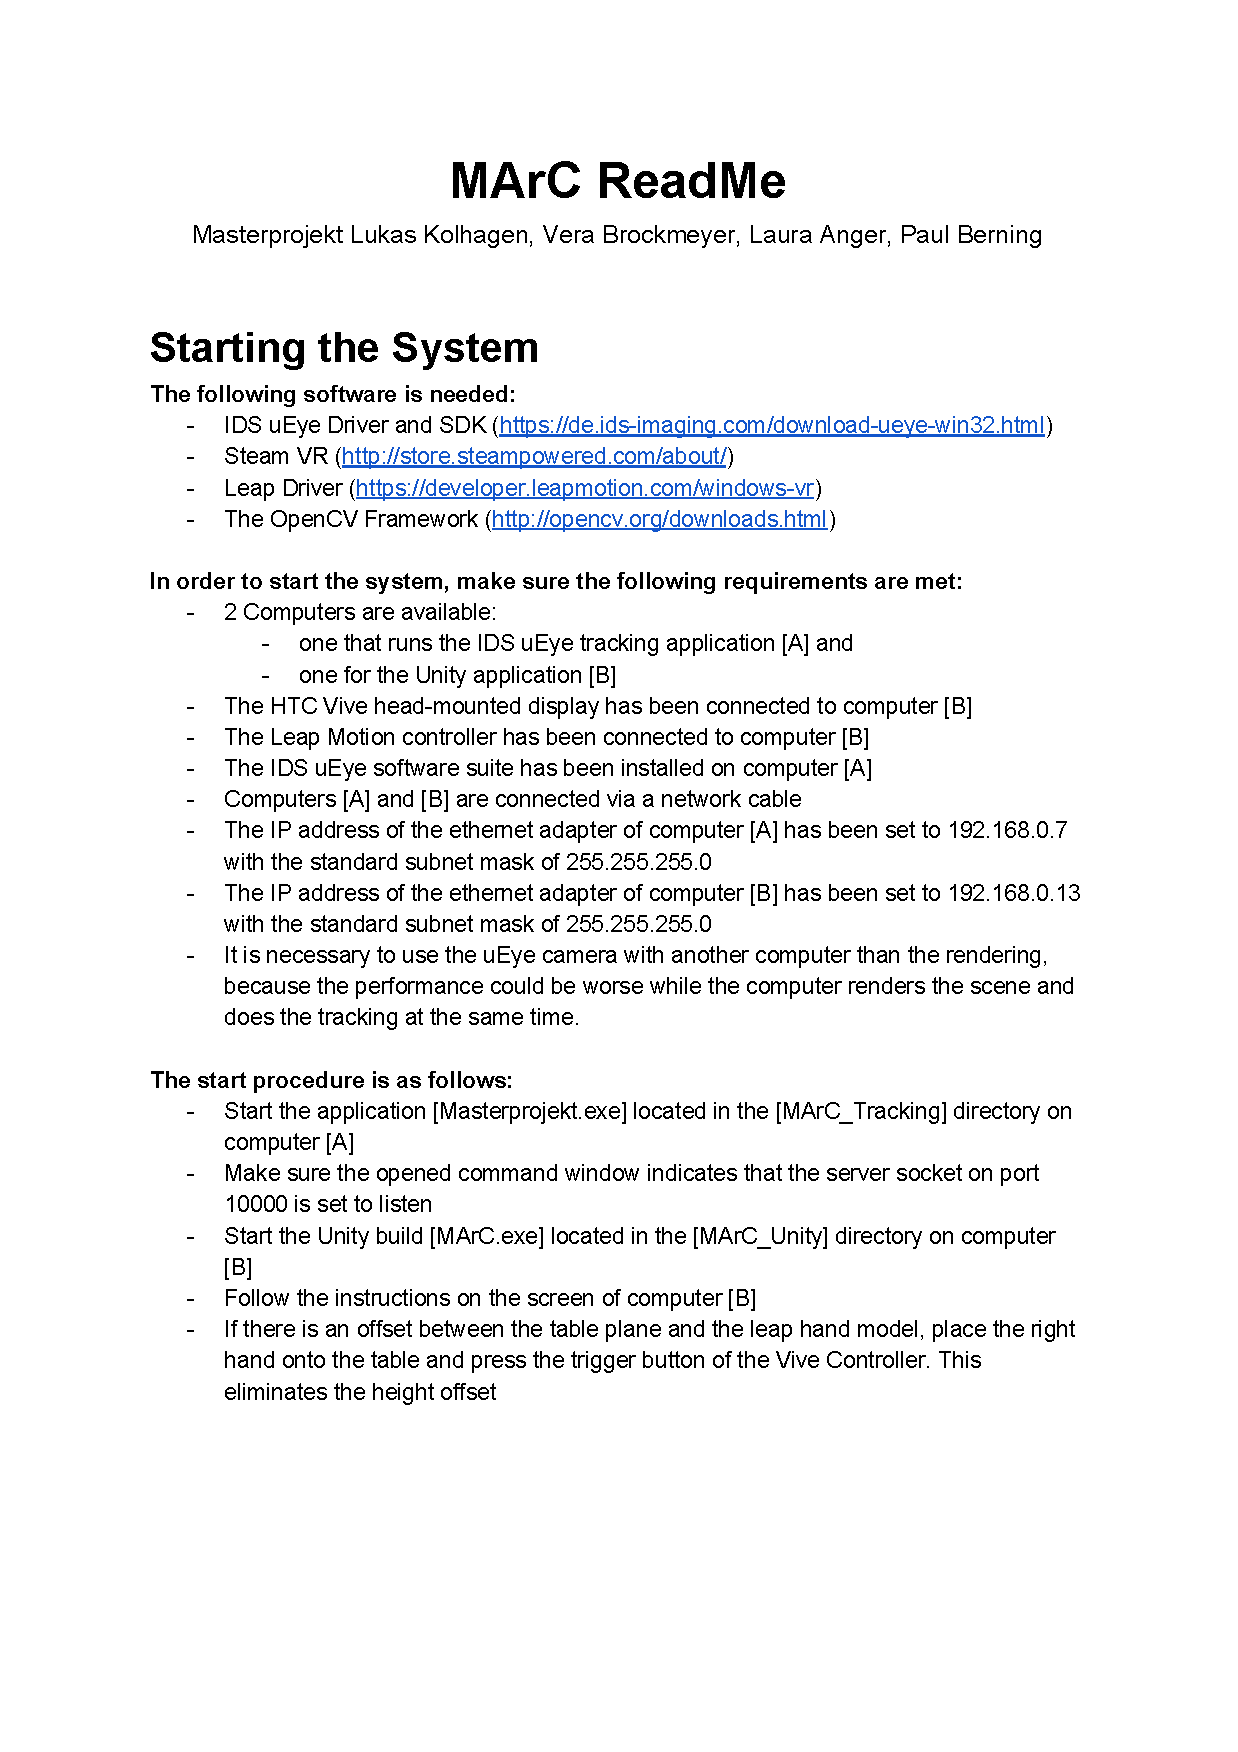
\includepdf[pages=-]{kapitel/anhang/ReadMe.pdf} 

\subsection{\texttt{startTCPServer()}-Methode}
\lstinputlisting[title=\lstname, caption={\texttt{startTCPServer()}-Methode in \texttt{TCP.cpp}}, label=lst:startTCPServer, language={C++}, linerange=22-77, firstnumber=22]{Quellcode/TCP.cpp}

\subsection{\texttt{interpretTCPMarkerData()}-Methode}
\lstinputlisting[title=\lstname, caption={\texttt{interpretTCPMarkerData()}-Methode in \texttt{readInNetWorkData.cs}}, label=lst:interpretData, language={[Sharp]C}, linerange=141-174, firstnumber=141]{Quellcode/readInNetworkData.cs}